
\chapter{FPGA y microprocesadores Soft-Core}
	

\section{FPGAs}

	\subsection{Introducción}
La fabricación de dispositivos semiconductores es un proceso complicado de plazos largos y costoso. Esto lleva a que los diseños destinados para la  implementacion en chip de silicio tengan poco oportunidad de ser prototipados antes de que comience la producción en grandes volúmenes. Esto supone una gran importancia  en las faces de prueba y verificación de un diseño antes de ser fabricado.

Basándose en la predicción de la ley de Moore donde expresa que aproximadamente cada dos años se duplica el número de transistores en un circuito integrado\cite{Etiqueta02}, Ross Freeman postulo que los transistores serian menos costoso cada año, haciendo asequible la fabricación de chips programables personalizables \cite{Etiqueta03}.
La compañía Xilinx, ofreció su primer chip en 1984 , que contiene arrays celdas lógicas (LCAs) , programables por el usuario en casi cualquier configuración que quisieran. Estos se conocen como Field Programmable Gate Array (\textit{FPGAs}) .

Las \textit{FPGAs} desempeñan un papel dual, uno como objetivo final de ejecución en un diseño y otro papel como prototipo para la implmentacion definitiva de un diseño. Su capacidad de reconfigurar el diseño parcial o totalmente para su actualización o corrección de errores tiene un costo relativamente bajo a diferencia del prototipado sobre ASICs.
Actualmente las \textit{FPGA} cuentan con una gran cantidad de recursos disponibles (Compuertas lógicas , Bloques de RAM) para implementar diseños digitales complejos.

Una desventaja de las \textit{FPGA}  es debido a la naturaleza inherente de las arquitecturas de \textit{FPGA}, los diseños implementados en \textit{FPGA} comparados con una ASICs en general tienen mas area, menos porformance y consumen mas energía.
		
	\subsection{Arquitecura}
Los componentes de una \textit{FPGA} se pueden dividir en cinco grupos:

\begin {itemize}
\item  Bloques lógicos configurables y \textit{Lookup Tables}.
\item  Bloques de entrada y salida.
\item  Bloques multiplicadores
\item  Bloques Manejadores de Clock Digitales.

 \end {itemize}



\begin{figure}[h!]
 \begin{center}
  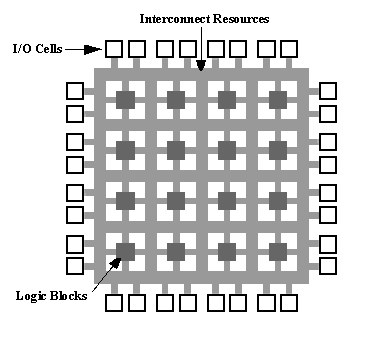
\includegraphics[width=0.5\textwidth,keepaspectratio=true]{./images/fpga1a}
  \caption{Etapas del modelo de desarrollo en espiral}
  \label{fig:esquema}
 \end{center}
\end{figure}

\section{Microprocesadores Soft-Core}
		\subsection{ IP-Core}
itro definición y licencias
		\subsection{Tipos de IP-Core}
			%\paragraph{\textcolor{orange}{ Tipos de IP-Core}}
		\subsection{Soft-Core}%%julius

